\chapter{Aplicação e ampliação da população: simulações com posições de catálogo}
\label{cap:c11-parcial}

A análise de aplicação auditou produtos públicos de PTA e executou uma extensão simulada com posições celestes de pulsares obtidas de catálogo público. As direções são observacionais; distâncias, sinais e ruídos são sintéticos. Nenhum tempo de chegada de pulso foi analisado. A campanha terminou com 596 realizações pareadas e 10.728 posteriores, após benchmark, piloto e referências funcionais diretas. A auditoria da geração e a conferência independente da agregação estatística passaram. As conclusões são condicionais aos parâmetros de ruído conhecidos e aos controles numéricos finitos descritos a seguir.

\section{Produtos públicos e o que eles permitem reconstruir}

O levantamento de 10 de setembro de 2026 distinguiu conteúdo efetivamente inspecionado, conteúdo declarado pelos depositantes e informação ainda não estabelecida. Foram consultados metadados, documentação e pequenos exemplos oficiais. O pacote MeerKAT de arquivos de timing foi adquirido e inventariado; os conjuntos grandes de cadeias e observações de outras colaborações não foram integralmente transferidos. Nenhum código externo consultado foi executado e nenhum TOA foi submetido à inferência deste trabalho.

O \href{https://zenodo.org/records/16051178}{NANOGrav15 timing, versão 2.1.0}, disponibiliza TOAs, modelos e produtos derivados, incluindo resíduos pós-ajuste. O produto \href{https://zenodo.org/records/21844115}{NANOGrav15 KDE, versão 2.0.0} fornece densidades espectrais marginais e frequências; não contém, por isso, a realização complexa conjunta necessária à análise A0. Suas notas de versão registram correções específicas, reforçando a necessidade de fixar o produto e a versão usados como referência. As \href{https://github.com/nanograv/15yr_stochastic_analysis/tree/a3e8b8776a646208ca2d307f83c20bc70e029933}{receitas oficiais de análise} ajudam a identificar benchmarks, mas uma cadeia de amplitudes espectrais ou parâmetros de uma ORF não equivale aos dados originais com fases e covariâncias preservadas.

A distribuição \href{https://docs.datacentral.org.au/meerkat-pulsar-timing-array/45-year/accessing-the-data/}{MeerKAT PTA de 4,5 anos} fornece TOAs e modelos de timing. O pacote inspecionado contém 83 arquivos PAR e 83 TIM. Ele não especificou, sozinho, toda a configuração estocástica necessária para reproduzir uma análise publicada: a ausência de opções de ruído num pacote não prova a ausência desses processos nas observações. As 32 sub-bandas descritas pelo produto são frequências eletromagnéticas de rádio, não 32 modos gravitacionais na série temporal. A descrição e a licença CC BY 4.0 foram conferidas no \href{https://api.datacite.org/dois/10.57891/j0vh-5g31}{registro DataCite do depósito}.

Os \href{https://zenodo.org/records/8300645}{dados EPTA DR2, versão 2.1}, contêm TOAs, modelos, relógios e configurações; as \href{https://zenodo.org/records/8091568}{cadeias EPTA GWB} são outro produto, condicionado à análise correspondente. O \href{https://ipta4gw.org/data-release/}{IPTA DR2} também oferece insumos de timing, embora a licença dos arquivos examinados não tenha sido estabelecida na auditoria realizada. Isso exige esclarecimento antes de eventual redistribuição, sem implicar impossibilidade de leitura ou inexistência de dados públicos.

Assim, a escolha de uma extensão simulada não decorre da falta de TOAs. O impedimento atual da aplicação observacional é a ausência de um adaptador validado para janela, timing, ruído e benchmark do conjunto escolhido. EPTA DR2new e NANOGrav15 foram identificados como candidatos a essa preparação futura, não como dados já analisados neste projeto.

\section{Contrato observacional e pseudocovariância}

No experimento Fourier usado nos capítulos anteriores, os coeficientes complexos são diretamente observados por definição, próprios e independentes entre frequências positivas. Um PTA real observa tempos de chegada irregulares. Um modelo mínimo é
\begin{equation}
 \boldsymbol d=M\,\delta\boldsymbol\xi+F\boldsymbol a+\boldsymbol n,
\end{equation}
em que $M$ representa o modelo linearizado de timing e $F$ a base amostrada nas datas reais. A marginalização e a modelagem dos processos estocásticos produzem uma covariância temporal $K(\theta)$. Relógios, efemérides, flags instrumentais, frequências de rádio, ruídos brancos, vermelhos e cromáticos fazem parte desse modelo.

Se $G^{\mathsf T}M=0$ e $D$ é uma transformação complexa fixa, então $\widetilde q=DG^{\mathsf T}\boldsymbol d$ possui
\begin{align}
 \widetilde C&=DG^{\mathsf T}KG D^\dagger,\\
 \widetilde P&=DG^{\mathsf T}KG D^{\mathsf T}.
\end{align}
Em geral, existem correlações entre frequências e pseudocovariância $\widetilde P\ne0$. Uma DFT ou a escolha de frequências $n/T$ não elimina essas propriedades. Se a projeção reduz o posto, a densidade deve ser formulada no suporte correto; acrescentar uma diagonal artificial não recupera a informação perdida.

Para explicitar a consequência, a representação real de $\widetilde q$ tem covariância
\begin{equation}
 K_R=\frac12\begin{pmatrix}
 \operatorname{Re}(\widetilde C+\widetilde P)&-\operatorname{Im}(\widetilde C-\widetilde P)\\
 \operatorname{Im}(\widetilde C+\widetilde P)&\operatorname{Re}(\widetilde C-\widetilde P)
 \end{pmatrix}.
\end{equation}
Para observações reais centradas e formas quadráticas simétricas $J_i$, os momentos são
\begin{equation}
 \mu_i=\operatorname{tr}(J_iK_R),\qquad
 \Sigma_{ij}=2\operatorname{tr}(J_iK_RJ_jK_R).
\end{equation}
Não se deve reaplicar a fórmula da CN própria sem considerar essa representação e sua normalização. Os estimadores quadráticos permanecem, em geral, não gaussianos.

A reconstrução de A exigiria os mesmos autos e pares, incluindo partes real e imaginária e todos os acoplamentos pertinentes. Uma compressão fixa preservaria $\mu_B=W\mu_A$ e $\Sigma_B=W\Sigma_AW^{\mathsf T}$; não bastaria somar blocos diagonais por frequência. C$_\beta$ e C$_{\rm full}$ deveriam usar exatamente o mesmo dado B, alterando a resposta e recalculando média e covariância. Resíduos embranquecidos, médias por época, covariâncias de parâmetros ajustados e posteriors espectrais não são produtos intercambiáveis com esse vetor observado.

Uma futura aplicação requer primeiro reproduzir um resultado publicado compatível com dataset, versão, seleção e ruído. Fixar uma média posterior de ruído como se fosse conhecida pode definir um estudo condicional, mas não reproduz uma análise que marginalizou conjuntamente esses parâmetros. Também será necessário validar a resposta no suporte das distâncias e frequências observacionais; a precisão de casos sintéticos com fases menores não se transfere automaticamente a pulsares a distâncias de quiloparsecs.

\section{Extensão simulada com populações aninhadas}

\begin{figure}[htbp]
\centering
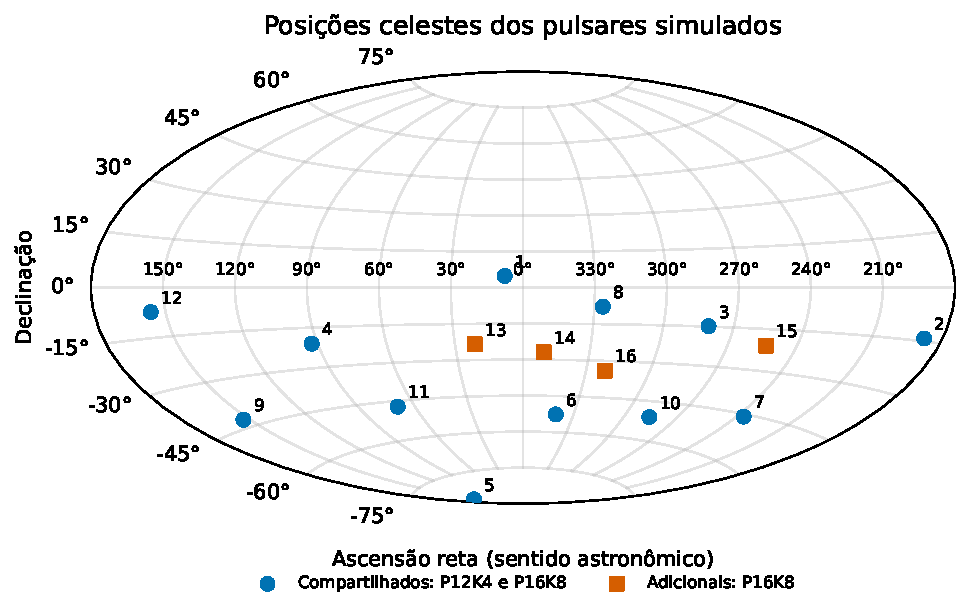
\includegraphics[width=\textwidth]{../figures/aplicacao/geometria_academica.pdf}
\caption{Direções públicas dos 16 pulsares selecionados do produto MeerKAT, com os 12 compartilhados por P12K4 e P16K8 e os quatro adicionais de P16K8. Os números correspondem à ordem determinística de seleção registrada nos metadados. Apenas as posições são observacionais: distâncias, sinais e ruídos usados no experimento são sintéticos. Fonte: metadados MeerKAT, DOI 10.57891/j0vh-5g31, CC BY 4.0; figura produzida neste trabalho.}
\label{fig:c11-geometria}
\end{figure}


O ramo executado compara P12K4 e P16K8: doze pulsares/quatro frequências e dezesseis pulsares/oito frequências. A geometria foi preparada a partir do \href{https://doi.org/10.57891/j0vh-5g31}{produto público MeerKAT}. Dos 83 PAR, 72 possuem RAJ/DECJ explícitos. Um algoritmo determinístico inicia no nome lexicograficamente primeiro e acrescenta a posição que maximiza a menor separação angular, com desempate lexicográfico. Nenhum resíduo ou resultado de inferência participa da seleção. Esse filtro de formato e a seleção angular não constituem amostra representativa da colaboração.

Os primeiros doze dos dezesseis pulsares formam o subconjunto P12. As posições públicas são tratadas como geometria fixa, sem nova solução de movimento próprio. Distâncias de 100--500 anos-luz, precisões nominais de 100--1000 ns e multiplicadores de ruído vermelho entre 0,5 e 2 são \emph{sintéticos}. Os valores dos pulsares compartilhados permanecem iguais nas duas configurações.

Ambas usam $T=4{,}5$ anos e $f_k=k/T$. Em P12K4, as dimensões são 48 coeficientes complexos em A0, 40 estimadores reais em A e 10 em B; em P16K8, são 128, 80 e 10. O máximo $fL/c$ passa de aproximadamente 397 para 889 ciclos. O último valor permanece dentro da faixa anteriormente testada na validação tensorial, e passou nos controles próprios descritos adiante. A comparação amplia simultaneamente a população e a banda; não separa causalmente o efeito de aumentar apenas uma delas.

Com nuisances conhecidos, a geração usou
\begin{equation}
 C_k(u)=P_{\rm GW}(f_k)\Gamma_k(u)+
 \operatorname{diag}\!\left[r_a^2P_{\rm red}(f_k)+2(\mathrm{EFAC}\,\sigma_a)^2\Delta t\right],
 \qquad q_k\sim\mathcal{CN}_{\rm pr\acute opria}(0,C_k).
\end{equation}
A cadência nominal é 14 dias, com $\Delta t=T/\lceil T/(14\,\mathrm{dias})\rceil$. Ela determina a potência branca do experimento periódico; não introduz uma janela real. Os parâmetros centrais são $(\log_{10}A_{\rm GW},\gamma_{\rm GW},\log_{10}A_r,\log_{10}\mathrm{EFAC})=(-15,13/3,-15{,}5,0)$, com índice vermelho individual quatro. A variável inferida é $u=f_gT$, uniforme em $[0,1]$.

A escala numérica por frequência foi comum aos canais compartilhados, usando a mediana das precisões da população 16, sem recalculá-la para P12. Nas unidades do experimento periódico, $C_k$ é uma PSD unilateral de resíduos em s$^3$, $q_k$ tem unidade s$^{3/2}$ e o coeficiente periódico é $q_k/\sqrt{2T}$. A conversão de massa é $m_gc^2=hu/T$; o suporte escolhido e seus quantis sem dados não representam uma restrição observacional.

Cada realização gerou um único vetor complexo de forma $8\times16$. P12K4 recebeu os quatro primeiros canais e os doze primeiros pulsares, sem novo sorteio. Sua covariância é a submatriz principal correspondente. Esse pareamento permite diferenças por realização, conservando a independência entre IDs de engenharia ou calibração.

\section{Controle gaussiano conjunto desenvolvido}

O controle G precisa preservar também a covariância cruzada entre estimadores das duas populações. Compartilhar uma semente entre duas fatorações arbitrárias não basta. Para cada frequência, escreva $C=LL^\dagger$ e $A_i=L^\dagger H_iL$. Seja $W$ uma matriz hermitiana aleatória com diagonal normal padrão real e elementos superiores $(x+iy)/\sqrt2$, com variáveis normais independentes. Define-se
\begin{equation}
 Y_i=\operatorname{tr}(H_iC)+\operatorname{tr}(A_iW).
\end{equation}
As coordenadas reais de $A_i$ na base hermitiana ortonormal são sua diagonal, $\sqrt2\operatorname{Re}A_{i,ab}$ e $\sqrt2\operatorname{Im}A_{i,ab}$ para $a<b$. Consequentemente,
\begin{equation}
 \mathbb E[Y_i]=\operatorname{tr}(H_iC),\qquad
 \operatorname{Cov}(Y_i,Y_j)=\operatorname{Re}\operatorname{tr}(H_iCH_jC).
\end{equation}
Incorporar os estimadores P12 com zeros no espaço de 16 pulsares e concatená-los aos P16 permite aplicar o mesmo vetor latente e obter a covariância conjunta correta. A construção continua válida para estimadores redundantes e uma covariância conjunta singular, sem jitter ou recorte de autovalores.

O componente foi verificado com covariâncias sintéticas: momentos, termos cruzados, orientação imaginária, estimadores nulos/duplicados e compressão linear. Uma revisão independente usou cubatura determinística em vez de repetir os sorteios do autor e encontrou erro absoluto máximo aproximadamente $1{,}60\times10^{-12}$. Esses testes verificam a álgebra do controle gaussiano; a validação da resposta física e da geração populacional é apresentada separadamente.

Os latentes CN e G usaram bancos independentes, condicionados à mesma massa. Dentro de G, A/B/C analisam o mesmo $Y$; a aproximação de resposta não altera a observação gerada. A normal conjunta reproduz os primeiros dois momentos do estimador CN, não sua distribuição inteira. A0 de P12 é marginal de A0 de P16, permitindo discutir informação esperada sob a priori; B16 e A\_G16 não determinam necessariamente os respectivos vetores P12. Não se exige ordenação dos limites superiores em realizações individuais.

\section{Desenho executado e alcance}

Foram realizadas nove análises por população: A0\_CN, A\_CN, B\_CN, C$_\beta$\_CN, C$_{\rm full}$\_CN, A\_G, B\_G, C$_\beta$\_G e C$_{\rm full}$\_G. As médias e covariâncias foram recalculadas para cada resposta. C$_\beta$ usa $\beta_1(u)=\sqrt{1-u^2}$ em todos os canais, preservando as escalas de fase $y_k=2\pi f_kL/c$; C$_{\rm full}$ usa a resposta física do primeiro canal, $\Gamma(\beta_1(u),y_1)$, em todos os canais. Ambas conservam a dependência da massa e preservam a potência e o ruído físicos. Todas as variantes de B usam a mesma observação comprimida.

O desenho prospectivo separou 500 massas da priori uniforme em $u$ de três células de 32 realizações: $u=0$ e $u=0{,}995$ com ruído central, e $u=0{,}5$ com ruído vermelho forte conhecido, $\log_{10}A_r=-14{,}7$. Os IDs 0--499 pertencem exclusivamente à calibração SBC; os 96 seguintes pertencem à recuperação condicional. A semente mestra é 20260912011, com bancos latentes independentes para CN e G e estados antes/depois de cada sorteio preservados.

Os 42 testes dos modelos corretamente especificados (A0\_CN, A\_G e B\_G, em duas populações) formam uma família Holm. Os 84 testes das aproximações formam outra, separada. Cada grupo inclui KS dos PITs de massa e logL, quatro coberturas unilaterais e a cobertura central de 90\%. Não se reivindica controle conjunto de erro familiar entre essas duas famílias. Todos os IDs permanecem nos denominadores; eventos não resolvidos recebem intervalo $[0,1]$.

\section{Benchmark numérico da geometria ampliada}

A decisão formal pelo ramo periódico simulado foi registrada em 12 de setembro de 2026, antes da execução física. O benchmark abrangeu 16 massas fixas, oito canais, duas resoluções harmônicas, oito casos independentes de integração direta no céu e seis controles de subconjunto ou rotação. As massas de engenharia não constituem amostra da priori para SBC.

A primeira tentativa foi interrompida por uma restrição do ambiente ao monitoramento de memória. A segunda identificou um erro de invariância de rotação de $4{,}58\times10^{-10}$ exclusivamente na diagonal. A recorrência de Legendre amplificava o arredondamento do produto escalar próprio. Para vetores unitários, $P_\ell(1)=1$ é uma identidade analítica; sua imposição apenas na diagonal elimina essa fonte de dependência da orientação sem alterar os termos fora da diagonal ou reparar autovalores da covariância. As tentativas anteriores foram preservadas e as tolerâncias permaneceram iguais.

O benchmark corrigido passou com diferenças máximas de $4{,}80\times10^{-12}$ entre resoluções, $6{,}14\times10^{-14}$ em relação à integração direta, $4{,}04\times10^{-12}$ nos limites analíticos e $4{,}18\times10^{-16}$ nos controles de subconjunto e rotação. Consumiu $110{,}78$ segundos de CPU; incluindo as duas tentativas anteriores, o consumo foi $221{,}30$ segundos. Esses controles validam os nós e casos finitos examinados, não uma precisão uniforme em todo o suporte de massa.

O piloto subsequente usa as 16 verdades fixas e as populações aninhadas P12K4/P16K8, com nove análises por população. Sua execução foi iniciada com limite cumulativo de 7200 segundos de CPU. O piloto terminou com 288 posteriores e 572.544 valores de verossimilhança. As 288 comparações de quadratura entre ordens, os 18 controles de refinamento independente e os 18 contrastes entre coordenadas passaram, assim como a comparação das CDFs interpoladas dos 288 alvos. A auditoria das 16 realizações reproduziu os estados aleatórios exatamente e encontrou erro escalado máximo de $3{,}22\times10^{-16}$ na reconstrução dos dados. A fase consumiu $693{,}16$ segundos de CPU, somando $914{,}47$ segundos com os benchmarks anteriores. As referências físicas diretas e a campanha subsequente são descritas abaixo; a aprovação não decorreu apenas do benchmark.


\subsection{Referências funcionais e campanha final}

As 18 referências diretas selecionadas antes do piloto cobrem os nove modelos nas duas configurações. Todos os quantis foram confirmados por integrais diretas em duas ordens, com respostas calculadas em duas resoluções harmônicas. Cinco eventos exigiram reduzir a massa das regiões de fronteira; as tentativas anteriores foram preservadas, sem relaxar as tolerâncias. Após esses refinamentos, os 18 controles passaram, e seus intervalos foram contidos pelos intervalos operacionais da rotina de síntese. Essa validação é finita e não prova ausência de cruzamentos em pontos não amostrados.

A rotina de síntese foi também aplicada às 288 posteriores do piloto: todas passaram nos controles de massa, enquanto 23 eventos permaneceram indeterminados e foram conservados com intervalo $[0,1]$. A campanha final foi iniciada com 500 realizações da priori uniforme em $u$ e três células de 32 realizações: $u=0$ e $u=0{,}995$ com ruído central, e $u=0{,}5$ com ruído vermelho forte conhecido. O total concluído é de 596 dados pareados e 10.728 posteriores. As famílias SBC, restritas às 500 realizações da priori, têm 42 testes de modelos corretamente especificados e 84 das aproximações, com correção Holm separada. A geração das 596 realizações foi reconstruída a partir das sementes nominais e dos estados aleatórios, com resíduo escalado máximo de $8{,}82\times10^{-16}$; o subconjunto complexo P12 foi reproduzido exatamente. A auditoria reutiliza o modelo de covariância, mas reconstrói explicitamente as flutuações hermitianas e os traços quadráticos.

\section{Resultados populacionais e informação}

A produção contabilizou 20.855.232 avaliações de log-verossimilhança, 500 novas massas verdadeiras e 15.000 novas matrizes de resposta; os nós de engenharia anteriores foram reutilizados. A diferença máxima entre as duas resoluções das novas respostas foi $4{,}80\times10^{-12}$. A execução final consumiu 233,56 segundos de CPU e 242,79 segundos de relógio, com pico de memória de aproximadamente 1,94 GiB. Esses tempos excluem preparação, piloto e referências diretas. A síntese posterior consumiu outros 659,64 segundos de CPU.

As 10.728 posteriores passaram nos controles operacionais de massa. Isso não implica resolução de todos os eventos de logL: os casos indeterminados foram conservados. Uma implementação separada reconstruiu a agregação dos intervalos, as contagens binomiais e o ajuste Holm, com 396 verificações aprovadas; a função de sobrevivência KS permanece a mesma biblioteca SciPy nas duas implementações. A validação funcional antecedente e essa auditoria de agregação têm escopos distintos.

\begin{table}[htbp]
\centering
\caption{Decisões SBC da população ampliada, condicionais aos intervalos numéricos operacionais. As famílias recebem ajustes Holm separados, a 5\%.}
\begin{tabular}{lrrr}
\hline
Família & Testes & Rejeições persistentes & Indeterminadas\\
\hline
Corretamente especificados & 42 & 0 & 3\\
Aproximações & 84 & 1 & 1\\
\hline
\end{tabular}
\end{table}

A rejeição persistente ocorre no KS do PIT de logL de A\_CN em P12K4, com limite superior do valor $p$ ajustado igual a 0,004956. O teste correspondente em P16K8 é indeterminado. Nos modelos corretamente especificados, as indeterminações são os KS de logL de A0\_CN nas duas populações e de A\_G em P12K4. Ausência de rejeição persistente não comprova equivalência, nem elimina uma incerteza numérica que permite rejeição. Os testes de massa não apresentam rejeição possível nos limites adotados após Holm.

\begin{figure}[htbp]
\centering
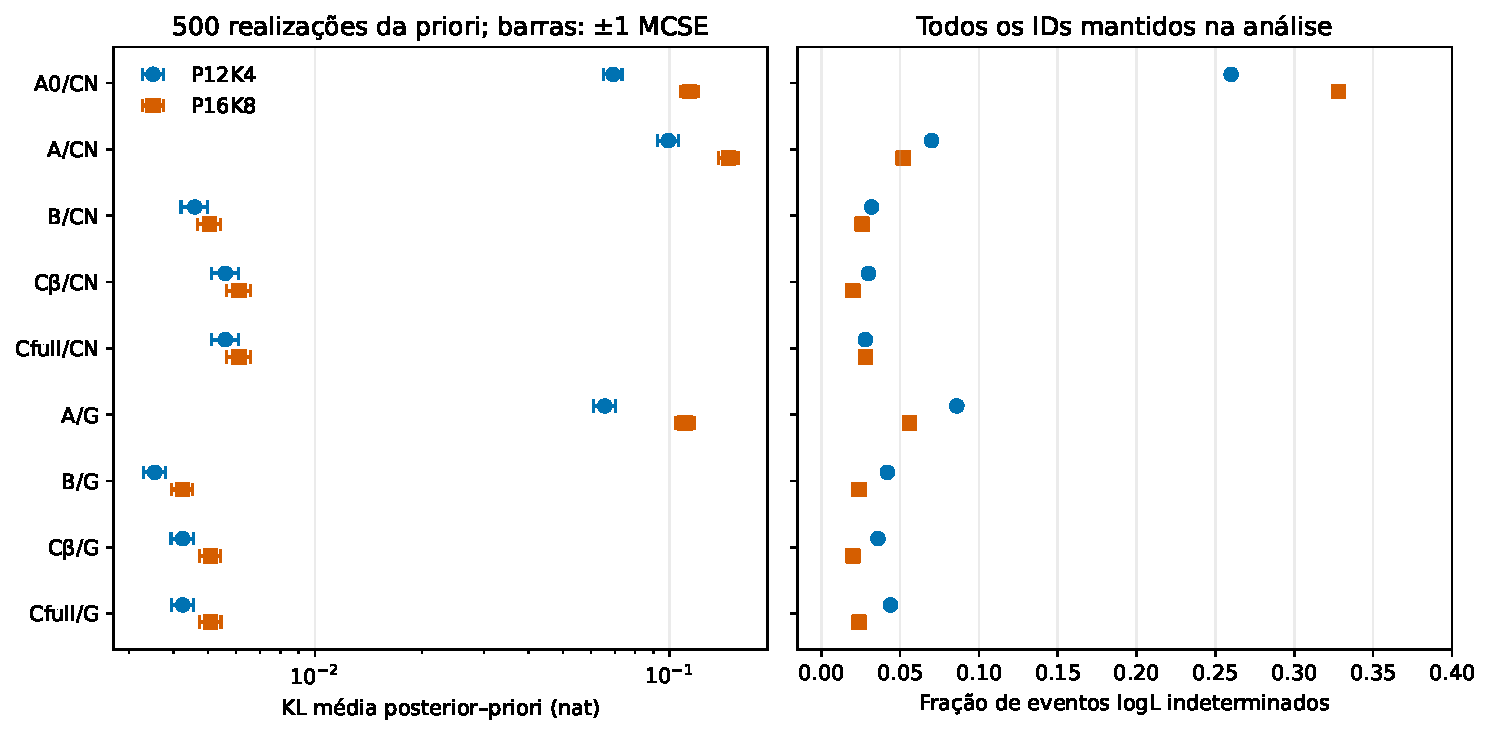
\includegraphics[width=\textwidth]{../figures/aplicacao/resultados.pdf}
\caption{Informação e resolução numérica nas 500 realizações da priori por grupo. À esquerda, média da divergência posterior--priori e erro Monte Carlo da média; à direita, fração de eventos de logL mantidos como indeterminados. Sob modelos aproximados, a KL é uma descrição da posterior calculada, não informação mútua do mecanismo verdadeiro. As barras não incluem erro sistemático numérico.}
\label{fig:c11-resultados}
\end{figure}

A comparação pareada A\_G menos B\_G fornece diferenças médias de KL de $0{,}06211\pm0{,}00477$ nat em P12K4 e $0{,}10631\pm0{,}00695$ nat em P16K8, onde o sinal $\pm$ indica um erro Monte Carlo da média sobre 500 realizações. Como o controle é gaussiano corretamente especificado e B é uma compressão fixa de A em cada população, essas médias estimam perda de informação esperada sob a priori. Não se exige ordenação da KL em cada realização. As 96 verdades fixas não entram nessas médias.

As posteriores comprimidas são pouco informativas neste desenho. A proximidade entre B e as variantes C pode, portanto, coexistir com pouco aprendizado sobre a massa; não autoriza usar uma resposta congelada em qualquer regime. A ampliação simultânea de pulsares e frequências tampouco identifica separadamente suas contribuições. Embora os coeficientes complexos P12 sejam subconjunto de P16, os respectivos estimadores angulares usam matrizes diferentes: não se presume que A ou B de P12 sejam compressões de A ou B de P16.

Nas três células fixas, as 32 realizações de cada modelo foram conservadas e as contagens de cobertura central foram propagadas como intervalos, com união dos intervalos binomiais. Para $u=0$, um intervalo central sob priori contínua exclui estruturalmente a fronteira; cobertura central zero nesse ponto não constitui falha de SBC nem da integração. Essas células são recuperação condicional, não amostras de calibração da priori.

\section{Contribuição e limites da aplicação}

A extensão conecta o experimento controlado a direções reais de um catálogo, mantendo um mecanismo gerador verificável. Ela amplia os testes metodológicos anteriores e mostra, no controle gaussiano, perda de informação por compressão; também identifica um desvio persistente da aproximação normal de estimadores quadráticos em uma configuração. Isso é consistente com a distinção entre momentos corretos e distribuição correta discutida nos capítulos anteriores. Os produtos públicos auditados continuam sendo candidatos a uma aplicação observacional futura, não benchmarks observacionais reproduzidos aqui.

Permanecem fora do alcance deste experimento: ajuste e marginalização de timing, amostragem irregular, distâncias observacionais com incerteza, inferência conjunta de ruídos e análise de TOAs. A precisão é sustentada por referências e refinamentos finitos, sem certificado uniforme de erro físico ou de ausência de cruzamentos não amostrados. Não há nova restrição observacional sobre a massa do gráviton.
